\secnumbersection{MARCO CONCEPTUAL}
    En este capítulo se desarrolla un estudio detallado a las técnicas de análisis y minería de textos más utilizadas en la literatura. Con esto, se busca poder tener una visión general de todos los alcances y usos que poseen los algoritmos en este campo, así como posibles aplicaciones al conjunto de datos que se estudiará posteriormente en esta memoria.
\subsection{Conceptos relevantes}
    Antes de comenzar a estudiar los algoritmos y metologías existentes en el área de minería y análisis de textos, se hace necesario conocer algunos conceptos relevantes dentro de esta disicplina. Esto, con la intención de entender el campo de estudio en dónde se desarrollará esta memoria.
    
\subsubsection{Minería de textos}
    Debido a la gran cantidad de textos que se producen hoy en día se estableció una disciplina que se preocupa de la extracción de información de estos activos, que pueden ser textos planos, archivos html o incluso pdf's.
    En general la disciplina minería de textos es definida como: el proceso de extraer patrones interesantes desde fuentes de textos para descubrir conocimiento. Para lograr esto la minería de textos aplica algoritmos de diversos campos tales como minería de datos, procesamiento de lenguaje natural e incluso de recuperación de la información \cite{yehia2016text}.
    Algunas de las tareas más recurrentes en proyectos de minería de textos son: 
    \begin{itemize}
        \item Extracción de información relevante desde un documento: esta tarea se puede efectuar extrayendo las \textit{keywords} de cierto documento o los tópicos que trata un conjunto de documentos.
        \item Extracción de entidades: dado un cierto documento es posible extraer las personas, organizaciones, lugares  o en general cualquier entidad que esté dentro del documento, con el fin de buscar relaciones entre documentos. Para esto se utilizan algoritmos de asociación, procesamiento de lenguaje natural, recuperación de información u otros.
        \item Clasificación de documentos según su contenido: la idea es que dado un conjunto de documentos etiquetados, poder etiquetar un nuevo documento cuya etiqueta no se conoce.
        \item \textit{Clustering} de documentos: dado un conjunto de documentos se busca encontrar grupos de documentos que sean lo más similares posibles. En general para medir similitud se utilizan algoritmos basados en distancias, usando la premisa de que si dos documentos son cercanos, es más posible que éstos se parezcan.
    \end{itemize}
\subsubsection{Procesamiento de Lenguaje Natural}
    Procesamiento de lenguaje natural ( NLP , por sus siglas en inglés), es un área de investigación en ciencias de la computación e inteligencia artificial preocupada del procesamiento de lenguajes naturales tales como inglés, español o chino mandarín. Este procesamiento generalmente involucra traducciones de lenguaje natural a números que un computador puede utilizar para aprender sobre el mundo. Este entendimiento del mundo es usado en ocasiones para generar textos de lenguaje natural que reflejan ese aprendizaje \cite{lane2019natural}. 
    
    En general el objetivo de NLP es diseñar algoritmos que permitan a un computador entender un lenguaje natural con la finalidad de realizar diversas tareas tales como \cite{NLP-DL}:
    \begin{itemize}
        \item Corrección de ortografía
        \item Búsqueda de palabras clave
        \item Búsqueda de sinónimos
        \item Traducciones
        \item Análisis semántico (¿Cuál es el significado de esta oración?).
    \end{itemize}
\subsection{Metodologías en Proyectos de Minería de Textos}
\subsubsection{Descubrimiento de conocimiento en bases de datos}
    Descubrimiento de conocimiento en bases de datos (KDD, por sus siglas en inglés), \cite{fayyad1996kdd} por sus siglas en inglés es un modelo utilizado en el desarrollo de proyectos de minería de datos. Según sus autores puede definirse como: el proceso no trivial de identificar, validar y comunicar patrones altamente entendibles y útiles ocultos en un conjunto de datos. En general, cuando se habla del proceso KDD existen 5 etapas  definidas, en dónde cada una depende del resultado de la etapa anterior (ver figura \ref{fig:KDD}). Sin embargo, en la descripción original del proceso, se describen 9 etapas las cuales se describen a continuación:

\begin{enumerate}
    \item \textbf{Comprensión del negocio}: se debe desarrollar un entendimiento del dominio y el conocimiento a priori relevante que se desea extraer luego del proceso KDD. Es importante que el objetivo planteado para el proceso KDD sea del punto de vista del cliente para que así se le pueda entregar valor al negocio en cuestión. 
    \item \textbf{Creación de un dataset objetivo}: se debe seleccionar el \textit{dataset}, un conjunto de variables o muestras de datos que serán utilizados para aplicar en etapas posteriores técnicas de minería de datos.
    \item \textbf{Limpieza de datos y preprocesamiento}: se deben eliminar el ruido de los datos si es necesario, manejar los registros con columnas faltantes y en general dejar el \textit{dataset} limpio para aplicar alguna técnica de minería de datos .
    \item \textbf{Reducción de datos y proyección}: En esta etapa se deben buscar las variables del \textit{dataset} más representativas dependiendo del objetivo de nuestro proyecto. Técnicas de reducción de dimensionalidad o técnicas de selección de características en general son usadas para extraer las características que utilizaremos en la siguiente etapa.
    \item \textbf{Enlazando los objetivos del proceso KDD a una técnica particular de minería de datos}: se busca relacionar los objetivos de negocio, definidos en la etapa [1], con el resultado que pueda tener alguna técnica de minería de datos dentro de los cuales pueden estar: Regresión, Clasificación y \textit{Clustering}.
    \item \textbf{Selecció del algoritmo de Minería de Datos}: En esta etapa el analista debe seleccionar los algoritmos de minería de datos que cumplan los objetivos planteados en la etapa anterior considerando los datos que se tienen para resolver el problema. 
    \item \textbf{Minería de Datos}: se deben buscar los patrones que puedan ser de utilidad para lograr el objetivo planteado en la etapa 1 
    \item \textbf{Interpretación de patrones encontrados}: Una vez aplicado los algoritmos de minería de datos se deben interpretar los patrones que el método haya encontrado. Para esto, en general, se aplican herramientas de visualización de datos dependiendo de la técnica que se haya utilizado.
    \item \textbf{Consolidando el conocimiento descubierto}: una vez encontrados e interpretados los patrones, el conocimiento adquirido puede ser consolidado de distintas formas como por ejemplo documentando y reportando a los \textit{stakeholders} del proyecto o simplemente agregándolo a otro sistema para futuras acciones.
\end{enumerate}

\subsubsection{Cross Industry Standard Process for Data Mining}
    La metodología Cross Industry Standard Process for Data Mining \cite{wirth2000crisp} (Crisp-DM por sus siglas), es una de las metodologías más utilizadas hoy en día en proyectos de minería de datos. 
    
    Crisp-DM propone dividir un proyecto de minería de datos en seis etapas en dónde además cada una de las etapas tiene subtareas asociadas que ayudan a completar cada etapa dependiendo del contexto y las condiciones de cada proyecto en particular. 
    
    \begin{figure}[H]
    \centering
    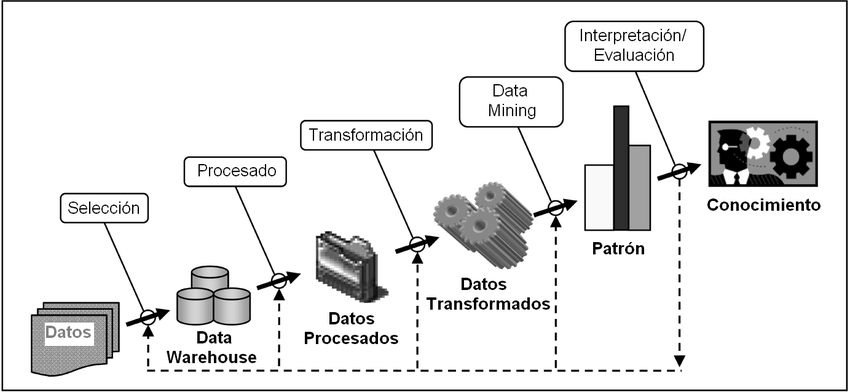
\includegraphics[width=0.8\textwidth]{The-Steps-of-a-KDD-process.png}
    \caption{\label{fig:KDD} Proceso KDD} Fuente: \cite{fayyad1996kdd}.
\end{figure}
    
    A continuación, se describen con un poco más de detalles cada una de las seis etapas de Crisp-DM \cite{wirth2000crisp}:
\begin{enumerate}
    \item \textbf{Comprensión del negocio}: el objetivo principal es comprender los objetivos y requisitos del proyecto desde una perspectiva empresarial con el fin de convertirlos en objetivos técnicos y en un plan de Proyecto. Crisp-DM propone 4 tareas para completar esta etapa:
    \begin{itemize}
        \item Determinar objetivos del negocio
        \item Evaluar la situación actual
        \item Determinar los objetivos del proyecto de minería de datos.
    \end{itemize}
    \item \textbf{Comprensión de los datos}: tiene como objetivo principal tener el primer acercamiento con los datos por parte del equipo de minería de datos. Para esto es común que se realicen análisis exploratorio de datos, detección de \textit{missing values} y cualquier tipo de evaluación que pueda entregar hipótesis sobre el estado de los datos. Para esta etapa, se propone completar las siguientes tareas:
    \begin{itemize}
        \item Recolectar datos iniciales
        \item Describir los datos
        \item Explorar los datos
        \item Verificar la calidad de los datos
    \end{itemize}
    \item \textbf{Preparación de los datos}: la idea es preparar los datos para ser luego utilizados por alguna técnica de minería de datos en la etapa de modelado.  Crisp-DM propone seguir las siguientes tareas para poder lograr todo este cometido:
    \begin{itemize}
        \item Seleccionar datos
        \item Limpiar datos
        \item Estructurar datos
        \item Integrar datos
        \item Formatear datos
    \end{itemize}
    \item \textbf{Modelado}: en esta etapa se espera que los expertos en minería de datos elijan un modelo que pueda cumplir los requisitos del problema planteado en la etapa de comprensión del negocio. Una vez implementado el modelo, este debe ser evaluado y analizado por los expertos  en minería de datos con el fin de poder ajustarlo en base a los datos que se poseen dentro de la compañía. En particular se proponen las siguientes tareas para la realización de esta etapa:
    \begin{itemize}
        \item Seleccionar la técnica de modelado
        \item Generar métodos de evaluación del modelo
        \item Construir el modelo
        \item Evaluar el modelo
    \end{itemize}
    \item \textbf{Evaluación}: Acá los expertos en el dominio analizan y evalúan los resultados del modelo producido en la etapa anterior. Esto se realiza teniendo en cuenta los criterios de éxito del problema definidos en la etapa número 1 como modo de validación del modelo empleado en la etapa número 4. Como en cada una de las etapas , Crisp-DM propone subtareas asociadas a la etapa de evaluación las cuales pasamos a definir a continuación:
    \begin{itemize}
        \item Evaluar los resultados
        \item Revisar del proceso
        \item Determinar los próximos pasos
    \end{itemize}
    \item \textbf{Implantación}: una vez que el modelo ha sido construido y validado, llega la hora de desplegar la solución generada. Para realizar esto, y dependiendo de la particularidad de cada proyecto, se pueden tomar acciones dentro del proceso de negocio que van desde recomendaciones del analista basadas en la observación y resultados del modelo. En general para realizar esto de buena manera Crisp-DM recomienda cumplir las siguientes entregas: 
    \begin{itemize}
        \item Plan de implantación
        \item Plan de monitoreo y mantención
        \item Informe final
        \item Revisión del proyecto
    \end{itemize}
\end{enumerate}
    
\subsubsection{Framework para Minería de textos según Dasri}
    \cite{dasritext} propone un \textit{framework} para desarrollar proyectos de minería de textos, el cual se puede resumir en tres pasos (Ver figura \ref{fig:Framework_TM} ): Preprocesamiento de textos, aplicación de técnicas de análisis de textos y Análisis de Textos. A continuación se describen cada una de las etapas:
    \begin{enumerate}
        \item \textbf{Preprocesamiento de Textos}: En general antes de aplicar cualquier técnica de minería de textos se deben realizar un par de tareas de preprocesamiento con el fin de obtener información más certera en la siguiente etapa del proyecto de minería de textos. Las tareas más recurrentes de preprocesamiento de textos son:
        \begin{itemize}
            \item Tokenización: Un documento es una colección de oraciones. En este paso se busca dividir la totalidad de las oraciones en su unidad más básica, es decir palabras. Para lograr esto se eliminan puntos , comas y espacios en blanco.
            \item Eliminación de \textit{StopWords}: En este paso se busca eliminar todos los \textit{tokens} obtenidos en el paso anterior que se identifiquen como \textit{stopwords}. Se conoce como \textit{stopwords} a las palabras que tienen una pequeña o ninguna significancia por si solas. En general cada idioma tiene una lista predeterminada de stopwords por ejemplo en inglés los más conocidos son: 'a’, 'is’, 'of’, 'an’, etc.
            \item Stemming: es la tarea de identificar la raíz de ciertas palabras. En la figura \ref{fig:Stemming} se puede apreciar como las palabras 'Jumps', 'Jumped' y 'Jumping' fueron sometidas al proceso de Stemming cuyo resultado final fue 'Jump.
        \end{itemize}
    \item \textbf{Técnicas usadas en minería de textos}: En esta etapa dependiendo del objetivo del proyecto de minería de textos se pueden utilizar técnicas y algoritmos que cumplan alguna de las siguientes tareas:
        \begin{itemize}
            \item Extracción de información
            \item Categorización
            \item \textit{Clustering} de textos
            \item Visualización de textos
            \item Resumen de textos
        \end{itemize}
    \item \textbf{Análisis de Textos}: en esta etapa se deben interpretar los resultados obtenidos luego de aplicar las técnicas de minería de textos, para así, poder extraer los patrones y el conocimiento implícito en el \textit{corpus} estudiado. Todo esto debe ser plasmado en un documento, que nos deberá mostrar los resultados finales del proyecto.
    \end{enumerate}
\begin{figure}[H]
    \centering
    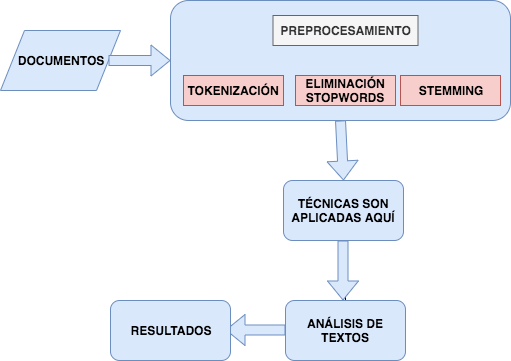
\includegraphics[width=0.8\textwidth]{Framework_TM.png}
    \caption{\label{fig:Framework_TM} \textit{Framework} para minería de textos según Dasri} Fuente: Text Mining Framework, Methods and Techniques \cite{dasritext}
\end{figure}

\begin{figure}[H]
    \centering
    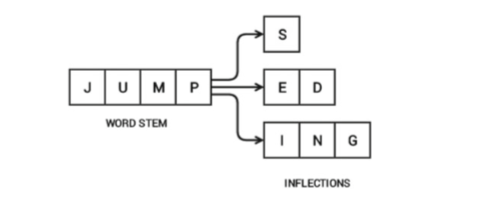
\includegraphics[width=0.8\textwidth]{figures/Stemming.png}
    \caption{\label{fig:Stemming} Proceso de \textit{Stemming}} Fuente: Text Analytics with Python \cite{sarkar2016text}
\end{figure}

    Una vez finalizados las dos etapas del proceso de minería de textos se deben interpretar las salidas de los algoritmos empleados en la etapa de aplicación de técnicas para así poder extraer los patrones y el conocimiento implícito en los documentos. Todo esto debe ser plasmado en un documento que nos deberá mostrar los resultados finales del proyecto.
    
\subsubsection{\textit{Framework} para en minería de textos según Kumar}
    \cite{kumar2014survey} propone un \textit{framework} para proyectos en minería de textos un poco más detallado que el descrito en la sección anterior. La metodología se compone en cinco etapas (ver figura \ref{fig:Framework_Ku}). A continuación se pasa a describir las etapas propuestas por kumar una por una:
    \begin{enumerate}
        \item \textbf{Preprocesamiento de textos}: al igual que en el marco de trabajo propuesto por Dasri, antes de realizar cualquier trabajo con los documentos éstos deben ser preprocesados. Para realizar esto se proponen las mismas tres etapas que proponía Dasri:
        \begin{enumerate}
            \item Tokenización
            \item Eliminación de \textit{stopwords}
            \item \textit{Stemming}
        \end{enumerate}
        \item \textbf{Transformación de textos}: se debe buscar una representación matemática para los textos que se están trabajando. En general existen dos posibles formas de representar textos de forma matemática: Bolsas de palabras o Vectores de Secuencia. Cada uno de estos métodos generan los \textit{features}, que posteriormente, serán consumidos por algún algoritmo de minería de textos.
        
        \item \textbf{Selección de características}: en esta fase se busca disminuir la cantidad de \textit{features} generadas en el proceso anterior. Para esto se busca eliminar las características consideradas como irrelevantes para los procesos de minería de textos. Una vez finalizada esta etapa el tamaño del \textit{dataset} a utilizar debería ser mucho más pequeño que al comienzo de la etapa, lo que implicará menores costos computacionales y espacio de búsqueda.
        \item \textbf{Aplicación de técnicas usadas en minería de textos}: En esta etapa Kumar propone lo mismo que Dasri, es decir  dependiendo de nuestro objetivo debemos seleccionar la técnica de minería de textos que cumpla alguna de las tareas comunes de la disciplina.

        \item \textbf{Evaluación de resultados}: tras la etapa anterior se deben analizar e interpretar los resultados. Además es vital utilizar métricas para evaluar el rendimiento de nuestros algoritmos como porcentajes de \textit{accuracy}, precisión, entre otras métricas útiles dependiendo de la técnica empleada.
    \end{enumerate}
    \begin{figure}[H]
    \centering
    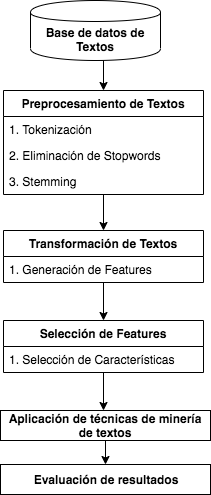
\includegraphics[height=0.7\textheight,width=0.5\textwidth]{figures/Framework_Kumar.png}
    \caption{\label{fig:Framework_Ku} Framework para minería de textos según Kumar} Fuente: A survey on text mining process and techniques \cite{kumar2014survey}
\end{figure}  

\subsubsection{Guía para proyectos de clasificación de Textos según Google}
    \cite{Google} propone un esquema de trabajo para enfrentar problemas de clasificación de textos de una forma un poco más técnica que los otros frameworks  estudiados hasta ahora. En esta guía, Google propone el siguiente flujo de trabajo (ver figura \ref{fig:Workflow_Google}) para un proyecto de clasificación de textos.
    \begin{figure}[h]
        \centering
        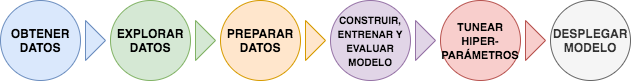
\includegraphics[width=0.8\textwidth]{figures/Workflow_Google.png}
        \caption{\label{fig:Workflow_Google} Flujo de trabajo para problemas de clasificación de textos según Google} Fuente: Text Clasification, Google Developers \cite{Google}
    \end{figure}
    A continuación, se describen cada una de las etapas del flujo de trabajo propuesto por Google:
    \begin{enumerate}
        \item \textbf{Obtener Datos}: para empezar, lo primero que se debe tener son textos. Según Google, los resultados de un proyecto de clasificación de textos dependen mucho de la calidad de los textos que se utilicen para entrenar cualquier tipo de modelo, por lo que este paso resulta vital.  En este caso Google indica que existen diversas fuentes para obtener textos tales como \textit{apis} de diversas compañías o incluso los propios textos que pueda tener la compañía patrocinadora del proyecto. En cualquiera de los casos anteriores Google indica que se deben tener las siguientes consideraciones a la hora de recolectar datos:
        \begin{itemize}
            \item Se debe intentar recolectar la mayor cantidad de textos para entrenar el modelo, ya que esto ayudará a generalizar de mejor forma los resultados.
            \item Se debe asegurar tener un \textit{dataset} balanceado, es decir intentar tener la misma cantidad de datos para cada clase a clasificar.
            \item Se debe intentar tener datos que cubran todos los casos posibles y no sólo usar con los casos comunes. 
        \end{itemize}
       \item \textbf{Explorar Datos}: una vez construido o obtenido un \textit{dataset}, es sumamente importante revisar que esté sea consistente con las expectativas del proyecto. Para realizar esto, se deben realizar revisiones aleatorios a los datos y ver, por ejemplo, si las etiquetas de estos corresponden a lo que se espera.
       Otra cosa relevante que se propone en esta guía es la revisión de ciertas métricas que permitirán determinar si el \textit{dataset} es apto para ser utilizado en un problema de clasificación de textos:
       \begin{itemize}
           \item Número de muestras
           \item Número de clases
           \item Número de clases por muestras
           \item Número de palabras por muestras
           \item Distribución de palabras según frecuencia
           \item Distribución de muestras según largo
       \end{itemize}   
      \item \textbf{Elección de un modelo}: una de las cosas más importantes a la hora de seleccionar un modelo de clasificación es resolver el \textit{trade-off} entre \textit{accuracy} y tiempo de cómputo. Para esto, Google desarrolló un algoritmo para seleccionar un modelo de clasificación de textos, el cual permite dependiendo, del \textit{dataset} seleccionar el modelo que permita encontrar el mayor accuracy en el menor tiempo posible. 

    \item \textbf{Prepararación de datos}: Tras la etapa anterior, es necesario llevar los datos a alguna representación numérica dependiendo del algoritmo a utilizar. Para realizar esto existen dos alternativas:
    \begin{itemize}
        \item Tokenización : dividir los textos en palabras u oraciones. Esto permitirá generalizar la relación entre los textos y las etiquetas asociadas a cada uno. 
        \item Vectorización : definir una buena medida numérica para caracterizar los textos.
    \end{itemize}
        En general, Google propone utilizar técnicas de tokenización en el caso de utilizar algoritmos basados en n-gramas. Por otro lado si se desean utilizar algoritmos secuenciales se sugiere utilizar técnicas de vectorización para representar los textos. 
        
        Una vez representados los datos de forma numérica se debe emplear alguna técnica de selección de características; para el caso particular de textos, Google propone utilizar las funciones de clasificación F y chi cuadrado.
    \item \textbf{Construir, entrenar y evaluar el modelo}: en esta etapa, Google propone formas y matices para construir, entrenar y evaluar el desempeño de una red neuronal con perceptrones multicapa y de una red neuronal recurrrente. 
    \item \textbf{Desplegar modelo}: esta etapa da algunos consejos con el fin de tener un buen rendimiento en producción del modelo generado una vez terminado el proyecto. A continuación, se describen los principales consejos descritos por Google:
    \begin{itemize}
        \item Se debe asegurar que los datos que serán evaluados con el modelo construido siguen la misma distribución que los datos usados para entrenar y validar el modelo.
        \item Regularmente se debe re-evaluar el modelo con nuevos datos adquiridos.
        \item Si la distribución de datos cambia, se debe reentrenar el modelo.
    \end{itemize}
    \end{enumerate}
    
\subsubsection{Comparación de metodologías de minería de textos}
    A continuación, se realizará una comparación entre las metodologías descritas en las secciones anteriores, con el fin de tener una visión general de que es lo que ofrece cada una. Para ello, se contruyo una tabla (Ver tabla \ref{table:comparación_metodologías_tm}), en dónde, las filas representan a etapas mencionadas dentro de la metodología, mientras que las columnas representan a una metodología en específico. El color achurado en la tabla indica si la metología, de la fila, menciona a la etapa, de la columna, como parte del proceso de minería de textos. En caso de que la metodología no presente a la etapa dentro del proceso descrito, se dejó el espacio en blanco dentro de la tabla.
    
    Si se analiza la tabla \ref{table:comparación_metodologías_tm}, se puede ver que las metodologías que realizan un desglose más detallado de las tareas generales que se realizan en un proyecto de minería de textos son las propuestas por Dasri y la propuesta por Google, siendo está última la que más detalles entrega en cómo enfrentar cada uno de los problemas, esto ocurre debido a que Google propone una guía por sobre una metodología. Por otro lado la metodología propuesta por Kumar salta varios pasos fundamentales para poder terminar con éxito un proyecto de minería de textos.

    \begin{table}[H]
    \centering
    \begin{tabular}{c|c|c|c|}
    \cline{2-4}
                                                       & Kumar                    & Dasri                    & Google                   \\ \hline
    \multicolumn{1}{|c|}{Preprocesamiento}             & \cellcolor[HTML]{DAE8FC} & \cellcolor[HTML]{DAE8FC} & \cellcolor[HTML]{DAE8FC} \\ \hline
    \multicolumn{1}{|c|}{Transformación}               & \cellcolor[HTML]{DAE8FC} &                          & \cellcolor[HTML]{DAE8FC} \\ \hline
    \multicolumn{1}{|c|}{Selección de Características} & \cellcolor[HTML]{DAE8FC} &                          & \cellcolor[HTML]{DAE8FC} \\ \hline
    \multicolumn{1}{|c|}{Aplicación de Modelo}         & \cellcolor[HTML]{DAE8FC} & \cellcolor[HTML]{DAE8FC} & \cellcolor[HTML]{DAE8FC} \\ \hline
    \multicolumn{1}{|c|}{Evaluación de Modelo}         & \cellcolor[HTML]{DAE8FC} & \cellcolor[HTML]{DAE8FC} & \cellcolor[HTML]{DAE8FC} \\ \hline
    \end{tabular}
    \caption{\label{table:comparación_metodologías_tm} Tabla comparativa metodologías en minería de texto.} Fuente: Elaboración Propia.
    \end{table}
    
\subsection{Preprocesamiento de textos}
    En general, cuando se desea analizar textos, es esperable que se pruebe algún algoritmo de minería de textos, cuyas entradas, en su mayoría, son elementos numéricos. Sin embargo, antes de poder realizar la transformación de textos a números, es necesario realizar algunos ajustes a los textos, pues los textos por naturaleza son datos no estructurados y poco estandarizados. En general, las técnicas de preprocesamiento buscan generar secuencias de componentes lingüísticos con una estructura y notación estándar, para así poder conseguir buenos resultados con alguna técnica en particular.
    
    En esta sección se describen las principales tareas y técnicas utilizadas a la hora de preprocesar textos. Para ello se utilizará el siguiente texto de juguete '' Nosotros discutimos brevemente sobre la sintaxis, estructura y diseño de filosofías.``    
\subsubsection{Tokenización de textos}
    Antes de poder hablar de tokenización de textos, es necesario definir que es un \textit{token}. Se entiende por \textit{token} a componentes independientes y mínimos textuales que por si sólos tienen una definida síntaxis y semántica \cite{sarkar2016text}. En general, se puede considerar como un \textit{token} a las oraciones que componen un párrafo o incluso a las palabras que componen una oración. 
    
    Ahora teniendo en cuenta qué es un token, se puede definir a la tokenización de textos como el proceso de romper un documento en sus respectivos \textit{tokens}, ya sean oraciones o palabras. A continuación, se utiliza el texto de juguete, definido anteriormente, para que quede claro el proceso de tokenización.
    
    
    \begin{table}[H]
    \centering
    \begin{tabular}{|c|c|}
    \hline
    \textbf{Texto en bruto}                                                                                                                & \textbf{Texto tokenizado}                                                                                                                                                                 \\ \hline
    \begin{tabular}[c]{@{}c@{}}``Nosotros discutimos brevemente \\ sobre la sintaxis, estructura \\ y diseño de filosofías.''\end{tabular} & \begin{tabular}[c]{@{}c@{}}[``Nosotros'', ``discutimos'', ``brevemente''\\  ``sobre'' ,``la'', ``sintaxis'',``estructura'' , ``y'', ``diseño'',\\  ``de'',  ``filosofías.'']\end{tabular} \\ \hline
    \end{tabular}
\end{table}

\subsubsection{Eliminación de caracteres especiales}
    Una tarea importante en el proceso de normalización de textos, es la eliminación de caracteres innecesarios y especiales. Estos pueden ser símbolos de exclamación, interrogación, puntuación e incluso etiquetas HTML en el caso de estar trabajando con datos extraídos directamente desde una página web. La principal razón de realizar este proceso es que a menudo estos caracteres no entregan mucha significancia cuando analizamos los textos utilizando técnicas de minería de textos o procesamiento de lenguaje natural.
    
    A continuación, se utiliza el texto de juguete para comprender el proceso de eliminación:
    
    \begin{table}[H]
    \centering
    \begin{tabular}{|c|c|}
    \hline
    \textbf{Texto tokenizado}                                                                                                                                                                     & \textbf{Texto sin caracteres especiales}                                                                                                                                                     \\ \hline
    \begin{tabular}[c]{@{}c@{}}[``Nosotros'', ``discutimos'', ``brevemente'', \\ ``sobre'' , ``la'', ``sintaxis'', \\ ``estructura'' , ``y'', ``diseño'', \\ ``de'',``filosofías.'']\end{tabular} & \begin{tabular}[c]{@{}c@{}}[``Nosotros'', ``discutimos'', ``brevemente'',\\  ``sobre'' , ``la'', ``sintaxis'', \\ ``estructura'' , ``y'',\\  ``diseño'', ``de'',``filosofías'']\end{tabular} \\ \hline
    \end{tabular}
    \end{table}
    
    Como se puede apreciar, el último token, ''filosofías.`` tenía un punto al final. Es por ello, que luego del proceso de eliminación de caracteres especiales, dicho punto fue eliminado.
    
\subsubsection{Eliminación de stopwords}
    El proceso de eliminación de \textit{stopwords} es uno de los principales en el proceso de normalización de textos. Se define un \textit{stopword} como aquellas palabras que prácticamente no poseen significado o utilidad por si solas. Algunos ejemplos de \textit{stopwords} son preprocisiones, pronombres, artículos e incluso algunos adverbios en español \cite{sarkar2016text}. 
    
    A continuación, se toma el conjunto de palabras que obtuvimos en la sección anterior y se aplica el proceso de eliminación de StopWords, con el fin de ver como disminuye el número de tokens a trabajar una vez efectuado este simple procedimiento:
    
    \begin{table}[H]
    \centering
    \begin{tabular}{|c|c|}
    \hline
    \textbf{\begin{tabular}[c]{@{}c@{}}Texto tokenizado,\\ sin caracteres especiales\end{tabular}}                                                                                               & \textbf{Texto sin stopwords}                                                                                                                                          \\ \hline
    \begin{tabular}[c]{@{}c@{}}[``Nosotros'', ``discutimos'', ``brevemente'', \\ ``sobre'' , ``la'', ``sintaxis'', \\ ``estructura'' , ``y'', ``diseño'', \\ ``de'',``filosofías'']\end{tabular} & \begin{tabular}[c]{@{}c@{}}[``Nosotros'', ``discutimos'', ``brevemente'',\\  ``sobre'' , ``sintaxis'', \\ ``estructura'' ,\\  ``diseño'',``filosofías'']\end{tabular} \\ \hline
    \end{tabular}
    \end{table}

    Una vez realizada la eliminación de \textit{stopwords} y la eliminación de caracteres especiales se logró disminuir el número de \textit{tokens} del texto original de 11 a 8. Osea que practicamente el 30\% de los \textit{tokens} no aportaban nada a posteriores análisis.

\subsubsection{Stemming}
    Para comprender el trabajo de \textit{Stemming}, primero se debe entender que una palabra en cualquier lenguaje es regularmente compuesta por su forma básica (\textit{stem}) más un afijo. Los afijos son unidades como los prefijos y sufijos cuya finalidad es unirlos a palabras en su forma \textit{stem} para cambiar su signficado \cite{sarkar2016text}. En la figura \ref{fig:Stemming} se puede ver como el \textit{stem} \textit{jump} puede ser cambiado a distintas formas agregandos diferentes afijos.
    
    A continuación, se utiliza la misma lista de \textit{tokens} que se obtuvo en la sección anterior, esta vez, transformandolos todos a su forma básica.
    
    \begin{table}[H]
    \centering
\begin{tabular}{|c|c|}
\hline
\textbf{Texto tokenizado}                                                                                                                                           & \textbf{Texto en stem}                                                                                                                                 \\ \hline
\begin{tabular}[c]{@{}c@{}}[``Nosotros'', ``discutimos'', ``brevemente'', \\ ``sobre'' , ``sintaxis'', \\ ``estructura'' , ``diseño'',,``filosofías'']\end{tabular} & \begin{tabular}[c]{@{}c@{}}[``Nosotr'', ``discut'', ``brevement'', \\ ``sobr'' , ``sintaxis'', ``estructur'' , \\ ``diseñ'',,``filosof'']\end{tabular} \\ \hline
\end{tabular}
\end{table}
    
    Como se puede apreciar, el principal problema del proceso de Stemming, es que las palabras resultantes no existen necesariamente en el diccionario. Esto implica que, a la hora de realizar análisis, es probable que  los resultados no sea faciles de interpretar ni comunicar.
    
\subsubsection{Lematización}
    El trabajo de Lematización es similar al proceso de Stemming con la diferencia que las palabras resultantes siempre estarán en el diccionario \cite{sarkar2016text}. El resultado del proceso de lematización de una palabra se conoce como el lema de ésta.  
    
    \begin{table}[H]
    \centering
\begin{tabular}{|c|c|}
\hline
\textbf{Texto tokenizado}                                                                                                                                           & \textbf{Texto en lema}                                                                                                                                     \\ \hline
\begin{tabular}[c]{@{}c@{}}[``Nosotros'', ``discutimos'', ``brevemente'', \\ ``sobre'' , ``sintaxis'', \\ ``estructura'' , ``diseño'',,``filosofías'']\end{tabular} & \begin{tabular}[c]{@{}c@{}}[``Nosotros'', ``discutir'', ``breve'', \\ ``sobre'' , ``sintaxis'', ``estructura'' , \\ ``diseño'',``filosofía'']\end{tabular} \\ \hline
\end{tabular}
\end{table}

    En general, dentro de las librerías existentes para lematizar, se debe indicar que tipo de palabra se lematizará. Esto hace el trabajo un poco más complicado ya que previo a poder lematizar \textit{tokens} estos deben estar etiquetados según su función en el contexto de la oración. Para solucionar esto a continuación, se describe la tarea Part of Speech (POS), la cual ayudará a solucionar este problema.
    
\subsubsection{Part of Speech}
    Part of Speech (POS) son categorías léxicas específicas a las cuales diversas palabras son asignadas acorde a su contexto sintáctico y rol dentro de un texto. Por ejemplo en inglés dependiendo del contexto la palabra ``Building'' puede ser un sustantivo o un verbo. 
    Los principales POS con que un token puede ser etiquetado dentro de un texto son verbo, sustantivo, adjetivo o adverbio en su infinidad de combinaciones. En la tabla \ref{table:Etiquetas_POS} se puede revisar las distintas etiquetas que se le pueden aplicar a los distintas palabras de un documento.

\begin{table}[h!]
\centering
\begin{tabular}{|l|l|l|}
\hline
Number & Tag   & Description                              \\ \hline
1.     & CC    & Coordinating conjunction                 \\ \hline
2.     & CD    & Cardinal number                          \\ \hline
3.     & DT    & Determiner                               \\ \hline
4.     & EX    & Existential there                        \\ \hline
5.     & FW    & Foreign word                             \\ \hline
6.     & IN    & Preposition or subordinating conjunction \\ \hline
7.     & JJ    & Adjective                                \\ \hline
8.     & JJR   & Adjective, comparative                   \\ \hline
9.     & JJS   & Adjective, superlative                   \\ \hline
10.    & LS    & List item marker                         \\ \hline
11.    & MD    & Modal                                    \\ \hline
12.    & NN    & Noun, singular or mass                   \\ \hline
13.    & NNS   & Noun, plural                             \\ \hline
14.    & NNP   & Proper noun, singular                    \\ \hline
15.    & NNPS  & Proper noun, plural                      \\ \hline
16.    & PDT   & Predeterminer                            \\ \hline
17.    & POS   & Possessive ending                        \\ \hline
18.    & PRP   & Personal pronoun                         \\ \hline
19.    & PRP\$ & Possessive pronoun                       \\ \hline
20.    & RB    & Adverb                                   \\ \hline
21.    & RBR   & Adverb, comparative                      \\ \hline
22.    & RBS   & Adverb, superlative                      \\ \hline
23.    & RP    & Particle                                 \\ \hline
24.    & SYM   & Symbol                                   \\ \hline
25.    & TO    & to                                       \\ \hline
26.    & UH    & Interjection                             \\ \hline
27.    & VB    & Verb, base form                          \\ \hline
28.    & VBD   & Verb, past tense                         \\ \hline
29.    & VBG   & Verb, gerund or present participle       \\ \hline
30.    & VBN   & Verb, past participle                    \\ \hline
31.    & VBP   & Verb, non-3rd person singular present    \\ \hline
32.    & VBZ   & Verb, 3rd person singular present        \\ \hline
33.    & WDT   & Wh-determiner                            \\ \hline
34.    & WP    & Wh-pronoun                               \\ \hline
35.    & WP\$  & Possessive wh-pronoun                    \\ \hline
36.    & WRB   & Wh-adverb                                \\ \hline
\end{tabular}
\caption{\label{table:Etiquetas_POS} Etiquetas POS.} Fuente: Alphabetical list of part-of-speech tags used in the Penn Treebank Project:
\cite{POS_Tag}
\end{table}

\subsection{Transformación de textos}
    Una vez finalizado el preprocesamiento de textos, es necesario transformar los documentos en un formato entendible para los diversos modelos de minería de textos que se aplicarán en etapas posteriores. Para realizar en general se ejecutan dos pasos:
    \begin{itemize}
        \item \textbf{Tokenización} : dividir el texto en palabras u oraciones. 
        \item \textbf{Vectorización} : definir una medida numérica para caracterizar cada token.
    \end{itemize}
    A continuación se describen dos métodos, que utilizando los pasos recién definidos, transforman los textos en elementos utilizables por algoritmos de minería de textos.
\subsubsection{Vectores de N-Gramas}
    En un vector de n-gramas, el texto es representado como una colección de únicos n-gramas. Se define a un n-grama como grupos de $n$ tokens adyacentes. Por ejemplo en la oración \textit{``The mouse ran up the clock''} los n-gramas para $n=1$ son \textit{['the', 'mouse', 'ran', 'up', 'clock']}, para $n=2$ son \textit{['the mouse', 'mouse ran', 'ran up', 'up the', 'the clock']}.
    
    Una vez finalizado el proceso de construcción de n-gramas, se debe buscar la manera de representarlos numéricamente. Por lo general, la estrategia a seguir es utilizar alguna métrica que permita cuantificar el impacto de cierto n-grama en algún documento. Para esto existen algunas estrategias ya planteadas las cuales se describen a continuación:
    \begin{itemize}
        \item \textbf{Codificación basada en frecuencias}: tal como dice el nombre, la estrategia a seguir en este tipo de vectorización es simplemente asignarle a cada uno de los n-gramas encontrados la frecuencia absoluta que este posee en el documento analizado.
        \item \textbf{Tf-idf}: es una técnica de vectorización extraída del campo de recuperación de la información. Esta técnica nace ya que por lo general existen ciertos n-gramas que aparecen con frecuencias absolutas muy parecidas entre distintos documentos. $Tf-idf$ es la multiplicación entre dos métricas importantes: frecuencias de términos y frecuencia inversa de documentos. A continuación se definen ambas métricas:
        \begin{enumerate}
            \item \textbf{Frecuencia de término}: es la frecuencia absoluta del término (n-grama) $i$ en el documento $j$. Se escribe como $tf$.
            \item \textbf{Frecuencia inversa en el documento}: Es la inversa de la frecuencia de documentos para cada término. Por lo que, se define a $idf$ como:
            \begin{equation*}
                idf(t) = 1+ log \left(\frac{C}{1+df(t)}\right)
            \end{equation*}
            Donde:
            \begin{itemize}
                \item $idf(t)$: Representa el $idf$ para el término $t$.
                \item $C$: Representa el número total de documentos en el corpus a analizar.
                \item $df(t)$: Representa el número de documentos en dónde el término $t$ aparece.
            \end{itemize}
    \end{enumerate}
    Como se mencionó anteriormente la métrica $tf-idf$ es la multiplicación de las dos métricas definidas anteriormente. Sin embargo a la hora de utilizarla se usa una versión normalizada , es decir, de la forma $\frac{tf-idf}{||tf-idf||}$.
   
    A modo de ejemplo, se calcularán vectores de un \textit{corpus} de documentos, basados en las dos estrategias definidas previamente. Para ello utilizaremos los siguientes textos: ``the sky is blue'', ``sky is blue and sky is beatiful'', ``the beautiful sky is so blue'' y ``i love blue cheese''.
    
    \begin{lstlisting}
    Usando frecuencia absoluta: 
   and  beautiful  blue  cheese  is  love  sky  so  the
0    0          0     1       0   1     0    1   0    1
1    1          1     1       0   2     0    2   0    0
2    0          1     1       0   1     0    1   1    1
3    0          0     1       1   0     1    0   0    0
    \end{lstlisting}
    \begin{lstlisting}
Usando tf-idf: 
        and  beautiful      blue    cheese        is      love       sky       so       the
0  0.000000   0.000000  0.399210  0.000000  0.488291  0.000000  0.488291  0.00000  0.603137
1  0.440516   0.347308  0.229880  0.000000  0.562351  0.000000  0.562351  0.00000  0.000000
2  0.000000   0.432026  0.285953  0.000000  0.349762  0.000000  0.349762  0.54797  0.432026
3  0.000000   0.000000  0.346182  0.663385  0.000000  0.663385  0.000000  0.00000  0.000000
    \end{lstlisting}
    Cada una de las filas de las matrices mostradas anteriormente representan un documento del \textit{corpus}, mientras que las columnas representan un n-grama presentes en el \textit{corpus} de documentos.  
    \end{itemize}
\subsection{Técnicas de minería y análisis de textos}
    Una vez finalizadas las etapas de preprocesamiento y transformación de textos, llega la hora de comenzar a extraer información de los datos en estudio. Para lograrlo existen varias tareas predefinidas en la literatura y más aún diversas técnicas que permiten resolverlas. A continuación se describirán algunas de las tareas más relevantes para el objetivo de esta memoria y las principales formas de resolverlas.
\subsubsection{Extracción de keywords en documentos utilizando n-gramas}
    Uno de los objetivos más importantes que se tienen a la hora de analizar textos es el de poder entender de qué habla el documento o el corpus a analizar. Para realizar esto, una de las formas más simples de hacerlo es encontrando las palabras o conceptos más relevantes dentro del documento. Para ser un poco más específico lo que se busca son los llamados  \textit{collocations}, un término traído desde el área lingüística el cual se puede definir como:  ``una secuencia o grupo de palabras que tienden a aparecer con frecuencia, tal que esta frecuencia es más que un hecho aleatorio'' \cite{sarkar2016text}. 
    
    Una forma de encontrar los \textit{collocations} más importantes de un documento en particular es utilizando n-gramas, ya definidos. Para esto se deben seguir dos pasos:
    \begin{enumerate}
        \item Encontrar los n-gramas 
        \item Rankear los n-gramas según algún criterio en particular
    \end{enumerate}
    El primer paso ya fue estudiado en extenso en la sección 2.4 por lo que ahora se procederá a explicar algunas métricas para rankear los n-gramas. La primera forma, y la más intuitiva quizás, para rankear los n-gramas es utilizando su frecuencia, es decir, se asume que los n-gramas que más aparecen en el documento serán los \textit{collocations} más importantes de este. A continuación se presenta un pequeño texto, al cual le extraeremos los 5 bigramas con mayor frecuencia absoluta.
    
    \begin{lstlisting}[language=Bash]
    """
        Elephants are large mammals of the family Elephantidae
        and the order Proboscidea. Two species are traditionally recognised,
        the African elephant and the Asian elephant. Elephants are scattered
        throughout sub-Saharan Africa, South Asia, and Southeast Asia. Male
        African elephants are the largest extant terrestrial animals. All
        elephants have a long trunk used for many purposes,
        particularly breathing, lifting water and grasping objects. Their
        incisors grow into tusks, which can serve as weapons and as tools
        for moving objects and digging. Elephants' large ear flaps help
        to control their body temperature. Their pillar-like legs can
        carry their great weight. African elephants have larger ears
        and concave backs while Asian elephants have smaller ears
        and convex or level backs.
    """
    \end{lstlisting}
    Del texto anterior, los 5 bigramas con mayor frecuencia son:
    \begin{lstlisting}[language=Bash]
    [('african', 'elephants'), ('elephants', 'large'), ('africa', 'south'), ('african', 'elephant'), ('animals', 'elephants')]
    \end{lstlisting}
    
    De lo anterior se  puede inferir que el texto que se está analizando habla sobre elefantes del sur de África. Ésto claramente es la idea más general del texto, y por ende nos entrega muy poca información. 
    
    Otra forma para rankear a los n-gramas encontrados es utilizando una medida llamada \textit{Información mutua puntual} (\textit{PMI} por sus siglas en inglés). El PMI puede ser calculado para dos tokens como el logaritmo del cuociente entre la probabilidad de que ambos \textit{tokens} aparezcan en el documento y la multiplicación de las probabilidades individuales de cada \textit{token}, asumiendo que ambas probabilidades son independientes \cite{church1990word}. La expresión matemática que define esta medida es:
    \begin{equation*}
        pmi(x,y) = log\left(\frac{p(x,y)}{p(x)p(y)}\right)
    \end{equation*}
    
    Aplicando esta métrica al texto analizado anteriormente, obtenemos los siguientes 5 bigramas:
    
    \begin{lstlisting}[language=Bash]
    [('africa', 'south'), ('body', 'temperature'), ('breathing', 'lifting'), ('carry', 'great'), ('control', 'body'), ('convex', 'level'), ('ear', 'flaps'), ('elephantidae', 'order'), ('extant', 'terrestrial'), ('family', 'elephantidae')]
    \end{lstlisting}
    De aquí se puede apreciar que el texto habla sobre elefantes y sus principales características. Esto entrega un poco más de información que sólo rankear los \textit{collocations} encontrados utilizando su frecuencia absoluta.
    
\subsubsection{Técnicas para la extracción de temas a partir de documentos}
    Otra de las tareas más recurrentes en proyectos de minería de textos es el de modelamiento de temas. La tarea consiste en que a partir de un \textit{corpus} de documentos se deben descubrir los temas del cual éste habla. En general los temas se presentan como un conjunto de conceptos, que tienden a estar frecuentemente juntos. A continuación se describen algunos de los algoritmos más conocidos para cumplir esta tarea:
    \begin{itemize}
\item \textbf{Latent Dirichlet Allocation}: \cite{blei2003latent} (LDA por sus siglas) es un modelo generativo probabilístico que ayuda a encontrar los temas latentes que se encuentran dentro de un \textit{corpus} de documentos. Para realizar esto se asume que cada documento es una combinación de tópicos, los cuales siguen una distribución de Dirichlet. LDA recibe como parámetros un conjunto de documentos, el número $k$ de tópicos a encontrar y los parámetros de concentración $\alpha$ y $\beta$. Una vez procesados todos estos elementos el algoritmo retorna (Ver figura \ref{fig:LDA_Model}) los tópicos encontrados en el corpus y la distribución de tópicos para cada uno de los documentos estudiados. Estos dos elementos los pasaremos a definir a continuación:
    
    \begin{itemize}
        \item \textbf{Tópico}: es formado como una distribución de palabras, en dónde cada palabra posee una probabilidad de pertenecer a dicho tópico.
        \item \textbf{Distribución de Tópicos}: Un documento es formado como una distribución de tópicos, en dónde cada tópico posee una probabilidad de pertenecer a dicho documento.
    \end{itemize}
    
    En la figura 6, se puede ver el algoritmo como una caja negra, en dónde entra una cierta colección de documentos, se seleccionan ciertos parámetros $\alpha$ y $\beta$ para luego entregar tópicos y una distribución de tópicos para cada uno de los documentos analizados.
    
    \begin{figure}[h]
        \centering
        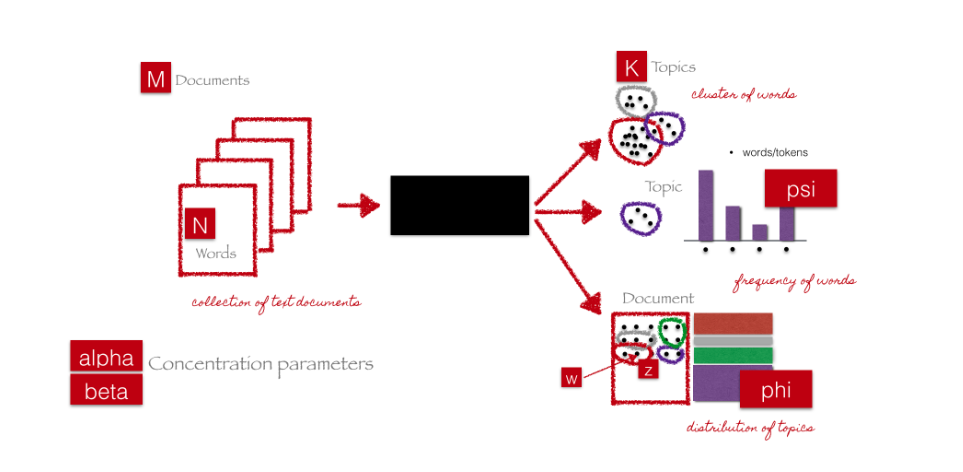
\includegraphics[width=1\textwidth]{figures/LDA.png}
        \caption{\label{fig:LDA_Model} Parámetros y Variables del Modelo} Fuente: Introduction to Topic Modeling in Python, PyGotham 2015 \cite{LDA_Model}
    \end{figure}
    
    Para realizar este trabajo LDA sigue el siguiente proceso iterativo:
    
    \begin{enumerate}
        \item Inicializa los parámetros $k$, $\alpha$ y $\beta$.
        \item Para cada documento, asigna aleatoriamente cada palabra a uno de los $k$ tópicos.
        \item Repetir los siguientes pasos hasta converger:
        \item Para cada documento $d$:
        \begin{enumerate}
            \item Para cada palabra $w$ en el documento:
            \begin{itemize}
                \item Para cada tópico $t$:
                \begin{itemize}
                    \item Calcular $P(t/d)$, la cual es la proporción de palabras en $d$ asignados al tópico $t$.
                    \item Calcular $P(w/t)$, la cual es la proporción de asignaciones al tópico $t$ sobre todos los documentos dada la palabra $w$.
                \end{itemize}
            \item Reasignar la palabra w con tópico t cuya probabilidad es $P(t/d) \cdot P(w/t)$ considerando todas las demas palabras y sus tópicos asignados.
            \end{itemize}
        \end{enumerate}
    \end{enumerate}
    
\item \textbf{Non-negative matrix factorization} (NNMF por sus siglas): es un algoritmo de factorización para matrices no negativas. Su principal diferencia con LDA es que es un algoritmo completamente determinista, o sea dada una serie de parámetros la sálida del algoritmo siempre es la misma. Formalmente se puede definir a NNMF como: Dada una matriz no negativa $V$, se deben encontrar dos matrices no negativas $W$ y $H$ las cuales multiplicadas aproximen V \cite{lee1999learning}. Matemáticamente esta representación es:
     
    \begin{equation*}
        V \approx WH
    \end{equation*} 
    Para obtener esta aproximación, usualmente se intenta disminuir alguna función de costo como la distancia euclídeana o la norma L2 entre las dos matrices, lo que es representado como:
    
    \begin{equation*}
        \text{argmin}_{\substack{W,H}} \frac{1}{2}||V-WH||^2
    \end{equation*}
    
    Si se considera la distancia euclideana como función de costo, lo anterior se resume a:
    
    \begin{equation*}
        \frac{1}{2}\sum_{i,j} \left( V_{ij} - WH_{ij} \right)^2 
    \end{equation*}
    
\item \textbf{Métricas para la evaluación de modelos} 
    Una de las tareas más importantes a la hora de realizar modelamiento de tópicos, es el de seleccionar el número correcto de tópicos a encontrar. Para ello, existen algunas métricas que nos ayudan a evaluar la calidad de los tópicos encontrados. A continuación se definen algunas de estas métricas:
    \begin{enumerate}
        \item \textbf{Coherencia}: la coherencia de los tópicos encontrados por un algoritmo \cite{mimno2011optimizing}, indica que tan coherentes son las palabras que se encuentran dentro de cada tópico. Para ello, se deben seleccionar las palabras más representativas dentro de cada tópico, y luego medir la ocurrencia y co-ocurrencia dentro del \textit{corpus} de documentos. La formulación matemática del índice de coherencia:
        \begin{equation*}
            Coherence(t) = \sum_{m=2}^M\sum_{i=1}^{m-1}\frac{\log{ D(w_m,w_t)+1}}{D(w_t)}
        \end{equation*}
        en donde:
        \begin{itemize}
            \item $M$ es la lista de las $M$ palabras más representativas del tópico t.
            \item $D(w_t)$ representa la ocurrencia de las palabra $w_t$ dentro del corpus.
            \item $D(w_m,w_t)$ la co-ocurrencia de la palabra $w_m$ y $w_t$ dentro del corpus.
        \end{itemize}
        \item \textbf{Coherencia CV}: La coherencia CV \cite{roder2015exploring}, es un índice que nos ayuda a cuantificar, que tan interpretables por los humanos son los tópicos encontrados por algún algoritmo en particular. Su dominio se encuentra entre 0 y 1, siendo 1 la configuración ideal de tópicos para cierto \textit{corpus}.
    \end{enumerate}
\end{itemize}
     
\subsubsection{Algoritmos de clustering de documentos}
    Dentro de las familias de algoritmos en minería de textos se encuentran los algoritmos de \textit{clustering}, cuyo objetivo es agrupar un conjunto de datos de tal forma que los datos que estén en el mismo grupo (llamado \textit{clúster}) sean lo más parecido unos a otros y lo más distinto a los datos que estén en otro \textit{clúster}. Dentro de los algoritmos de \textit{clustering} existen al menos dos distintas categorías:
    \begin{itemize}
        \item \textbf{Clustering jerárquico}: este tipo de clustering se basa en el concepto que objetos similares son cercanos entre sí y lejanos a los objetos distintos en el espacio vectorial dónde son representados. Clusters son formados conectando objetos basados en su distancia y pueden ser visualizados usando un dendograma.
        
        \item \textbf{Clustering basado en centroides}: este tipo de clustering se construye de tal forma que cada cluster posee un centroide el cual es el miembro más representativo del cluster y además posee las características que distinguen el grupo encontrado del resto de los datos.
    \end{itemize}
    A continuación se describen los principales algoritmos de \textit{clustering} de cada una de las categorías descritas anteriormente.
\paragraph{Clustering jerárquico aglomerativo} 
\paragraph*{}Dentro del clustering jerárquico existen dos estrategias distintas para realizarlo:
    \begin{itemize}
        \item \textbf{Aglomerativo}: sigue una aproximación \textit{bottom-up}. Esto quiere decir que se comienza con todos los puntos en distintos \textit{clusters} y a medida que el algoritmo avanza se van uniendo hasta formar un único \textit{cluster} que contiene a todos los datos.
        \item \textbf{Divisivo}: al contrario del \textit{clustering} aglomerativo, sigue una aproximación top-down. Esto quiere decir, todos los puntos comienzan como un único \textit{cluster} y a medida que se avanza en el algoritmo, dichos \textit{clusters} son separados.
    \end{itemize}
    Para un \textit{clustering} de este tipo es necesaria la definición de dos métricas: Distancia entre puntos y criterio de enlace entre \textit{clusters}. Para ello se definen algunos de los criterios de enlace entre \textit{clusters} más utilizados en la literatura:
    
    Dados dos clusters, $P$ y $Q$ se definen los siguientes criterios de enlace:
    \begin{itemize}
        \item \textbf{Single Link}: 
        \begin{align*}
          d(P,Q) &= \min_{\substack{x \in P\\
                  y \in Q}}
        d(x,y) 
        \end{align*}
        \item \textbf{Complete Link}:
        \begin{align*}
          d(P,Q) = \max_{\substack{x \in P\\
                  y \in Q}}
        d(x,y) 
        \end{align*}
        \item \textbf{Group Average}:
        \begin{align*}
            d(P,Q) = \frac{1}{|P|\cdot|Q|} \sum_{\substack{x \in P\\
            y \in Q}}
            d(x,y)
        \end{align*}
        \item \textbf{Ward’s method}:
        \begin{align*}
            d(P,Q) &= \Delta SSE \\
            d(P,Q) &= \sum_{z \in P \cup Q} ||z-c_{P \cup Q}||^2- \left[\sum_{x \in P}||x-c_p||^2+\sum_{y \in Q}||y-c_q||^2\right] \\
            d(P,Q) &= \frac{|P|\cdot|Q|}{|P|+|Q|}||c_p-c_q||^2 
        \end{align*}
    \end{itemize}
    Utilizando alguno de dichos criterios de enlace más alguna medida de distancia se puede realizar un proceso de \textit{clustering} aglomerativo. 
    
    Algunas de las medidas de distancias más utilizadas en este tipo de algoritmos son:
    
    \begin{itemize}
        \item \textbf{Distancia Euclídeana}: o L2,  es definida como la distancia más corta que puede existir entre dos puntos. Matemáticamente se puede expresar como:
        \begin{equation*}
            d(p,q) = d(q,p) =\sqrt{\sum_{i=1}^n\left(q_i-p_i\right)^2}
        \end{equation*}
        \item \textbf{Distancia de Jensen Shannon}: propuesta como un método para medir la similitud entre dos distribuciones de probabilidad \cite{endres2003new}. Una definición de esta métrica es: Sean P y Q dos medidas de probabilidad, entonces se define la distancia de Jensen Shannon como:
        \begin{equation*}
        J(P,Q) = \frac{1}{2}\left(D(P||R)+D(Q||R)\right)
        \end{equation*}
        con $R=\frac{1}{2}(P+Q)$ y $D(\cdot||\cdot)$ es la divergencia Kullback-Leibler.
        \item \textbf{Distancia de Manhattan}: o L1, es definido como el camino más corto desde un punto $a$ a uno $b$ tomando solo rutas verticales u horizontales. Matemáticamente se expresa como:
        \begin{equation*}
            MD(u,v) = \sum_{i=1}^n \left|u_i - v_i\right|
        \end{equation*}
    \end{itemize}
    
\paragraph{Clustering basado en centroides}
\subparagraph{Algoritmo K-means}
\subparagraph*{}
    Uno de los algoritmos más famosos para realizar \textit{clustering} basado en centroides es el algoritmo k-means. K-Means tiene como entrada el número $k$ de clusters que deseamos encontrar y los datos por supuesto.  Para entender mejor el algoritmo, enseguida se describe:
    \begin{lstlisting}
        Select k points as initial centroids.
        repeat
            Form k clusters by assigning each object to its closest centroid.
            Recompute the centroid of each cluster.
        until Centroids don't change or iterations.
    \end{lstlisting}
    Algunos elementos a considerar son :
    \begin{itemize}
        \item Los centroides iniciales son escogidos de forma aleatoria.
        \item El centroide de cada \textit{cluster} es la media aritmética de todos los elementos pertenecientes al mismo.
        \item La cercanía entre puntos es calculada usando la distancia euclideana.
    \end{itemize}
\paragraph{Métricas para la evaluación de clusters}
\paragraph*{}
    Para medir la calidad de los \textit{clusters} encontrados, existen dos grupos de métodos: intrínsecos y extrínsecos. Los primeros miden que tan separados están los clústers entre sí. Por otro lado los métodos extrínsecos son utilizados cuando ya se conoce la agrupación de los datos que se tienen disponibles, es decir, sirven para probar algoritmos de clustering sobre datos donde ya se conoce la agrupación óptima. Para efectos de esta memoria, como no se conoce la configuración óptima de agrupaciones, se considerarán sólo describir métodos íntrinsecos, siendo uno de ellos el coeficiente de Silhoutte.
    
    \begin{itemize} 
    \item \textbf{Coeficiente de Silhoutte}:
    Sea un \textit{dataset} $D$ de $n$ datos. Suponiendo que se generaron K \textit{Clusters}, $C_1,C_2,...,C_k$. Para cada dato $o \in D$, se calcula $a(o)$ como qué tan compacto está el clúster $C_i$ que contiene a $o$  definido de la siguiente forma:
    
    \begin{equation*}
        a(o) = \frac{\sum_{o' \in C_i, o \neq o'}dist(o,o')}{|C_i| - 1 }
    \end{equation*}
    Luego se define $b(o)$, como el grado de separación, del dato $o$ respecto a los demás clusters.
    \begin{equation*}
        b(o) = \min_{C_j:1\leq j \leq k, j \neq i} \frac{\sum_{o' \in C_j}dist(o,o')}{|C_j|}
    \end{equation*}
    Finalmente. se define el coeficiente de silhouette \cite{rousseeuw1987silhouettes} como:
    \begin{equation*}
        s(o) = \frac{b(o) - a(o)}{max\{a(o),b(o)\}}
    \end{equation*}
    El coeficiente de Silhouette posee un dominio entre -1 y 1. Siendo 1 la configuración óptima, ya que asegura que un dato está bien cohesionado con su cluster y al mismo tiempo bien alejado de los otros clusters. Por otro lado, cuando el coeficiente de Silhoutte es -1 indica que el dato está cercano a otros \textit{clusters} y no bien cohesionado con su \textit{cluster}, por ende se tiene una mala configuración.
    
    El promedio del coeficiente de Silhoutte para todos los puntos dentro del \textit{dataset} a estudiar, indica qué tan buena es la configuración. Por lo que, se puede utilizar este índice para seleccionar el número adecuado de clusters a encontrar para cierto algoritmo. \end{itemize}

\subsubsection{Técnicas de visualización de textos}
    Una de las cosas más complejas que se debe realizar a la hora de ejecutar un proyecto de minería de textos es el de visualizar estos datos. Esto ocurre debido a que la mayoría de las herramientas de visualización trabajan con datos numéricos por lo que utilizar estas herramientas en el caso de textos no es algo tan natural. 
    
    Las técnicas de visualización de textos tienen muchas aplicaciones que van desde presentar resultados a los \textit{stakeholders} de nuestro proyecto de minería de textos hasta ser una herramienta de ayuda a la hora de seleccionar un modelo para trabajar sobre los datos.
    
    En las siguientes subsecciones, se describen algunas de las tareas más frecuentes a la hora de visualizar textos. Esto va, desde visualizar el comportamiento de ciertos conceptos en un documento particular hasta entender como varía dicho el uso de dicho concepto en un \textit{corpus}.

\paragraph{Análisis visual de características}
\paragraph*{}
    En proyectos de minería de datos es natural utilizar muchas técnicas de visualización para realizar tareas de selección de características, reducción de dimensionalidad e incluso encontrar patrones de forma visual. Dentro de estas técnicas en bajas dimensiones se encuentran visualizaciones tales como \emph{Pairwise Correlation HeatMaps y Barplots} que son utilizados para, por ejemplo, explicar la varianza de cada \textit{feature} y en lo posible encontrar correlaciones entre variables.
    
    Por otro lado en proyectos de minería de textos estas herramientas no son tan fáciles de utilizar por lo que se debe recurrir a otras técnicas para tener los primeros acercamientos con nuestros datos, tales como visualización de n-gramas, visualización de un temas y clustering de documentos.
    
\subparagraph{Visualización de N-Gramas}
\subparagraph*{}
    Como se revisó anteriormente una de las formas de representar un texto es utilizando n-gramas. Considerando que existen muchos n-gramas que se repiten a lo largo de un texto se pueden realizar diversas visualizaciones con esta agrupación de datos y su frecuencia.
\begin{enumerate}
    \item \textbf{Frecuencia de n-gramas a lo largo del tiempo}:
        considerando un \textit{corpus} de documentos y su fecha de emisión se puede construir una visualización que permita ver como ha variado la cantidad de menciones a cierto n-grama a lo largo del tiempo. A modo de ejemplo (ver figura \ref{fig:NgramasTiempo}), se puede ver como ha variado la cantidad de menciones sobre Donald Trump, Bernie Sanders y Hillary Clinton a lo largo del 2016. Para ello se tomó como corpus a estudiar los tweets emitidos en dicho año.
    \begin{figure}[H]
        \centering
        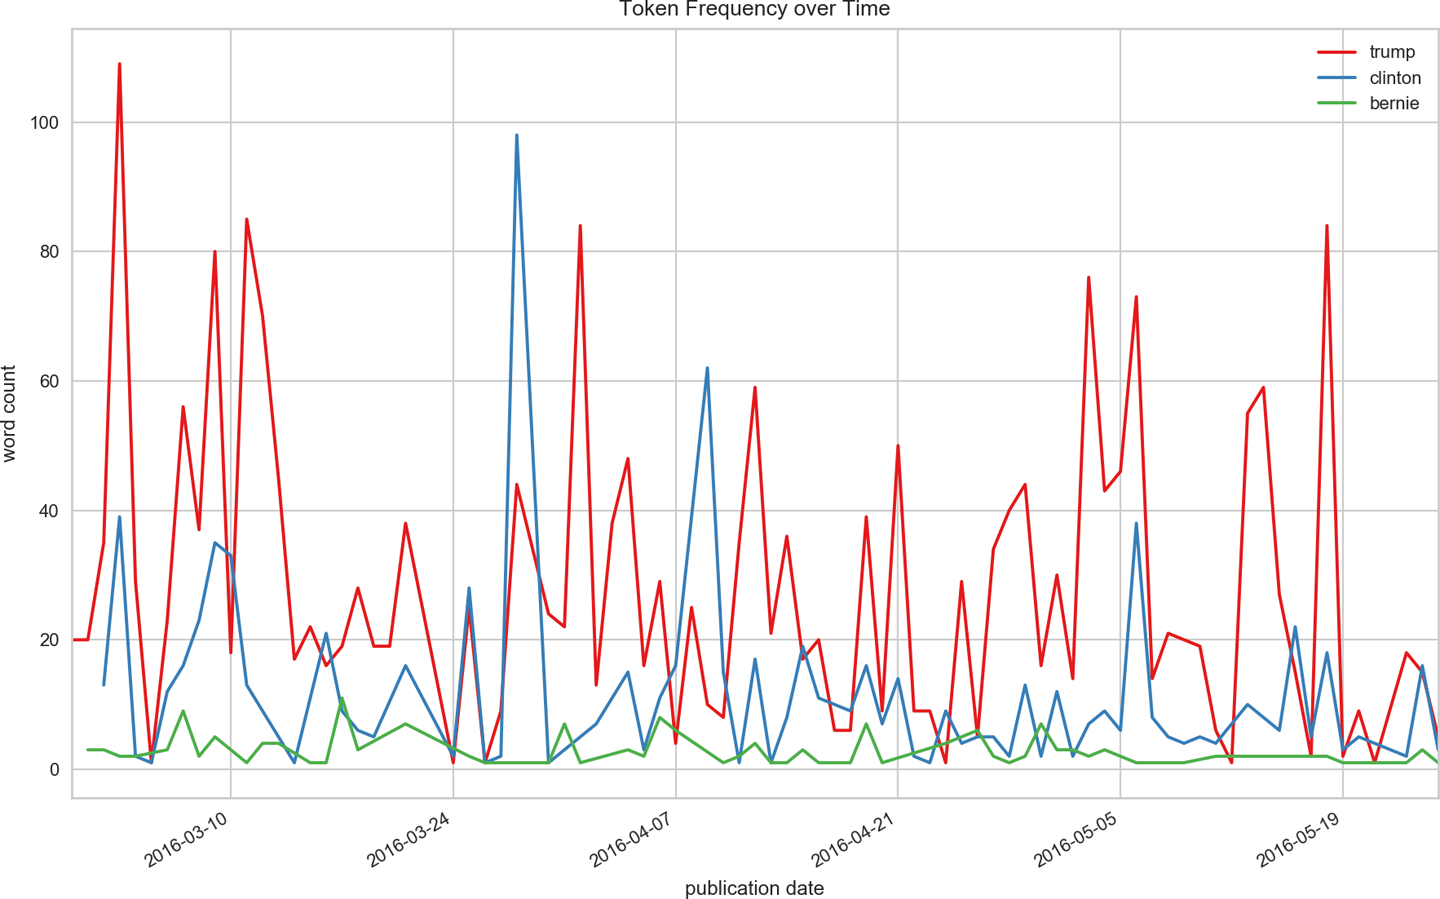
\includegraphics[width=0.8\textwidth]{figures/Frecuencia_sobre_tiempo.png}
        \caption{\label{fig:NgramasTiempo} Frecuencia de n-gramas a lo largo del tiempo} Fuente: Applied text analysis with python \cite{bengfort2018applied}
    \end{figure}
    \item \textbf{Dispersión léxica}: algo interesante que podemos visualizar dentro de un único documento es como los n-gramas más importantes aparecen y desaparecen. Para realizar esto se utilizan los gráficos de dispersión léxica (Ver figura \ref{fig:Lexical} ). A modo de ejemplo se puede ver como las palabras sobre conspiración que más utiliza Donald Trump en sus tweets han variado a lo largo de los años. Para ello en el eje Y, se listaron todas las palabras relacionados a conspiración. Luego en el eje X se listó la fecha de emisión de cada uno de los tweets estudiados, para finalmente, marcar con un punto los tweets que utilizaban dicho concepto.
    \begin{figure}[H]
        \centering
        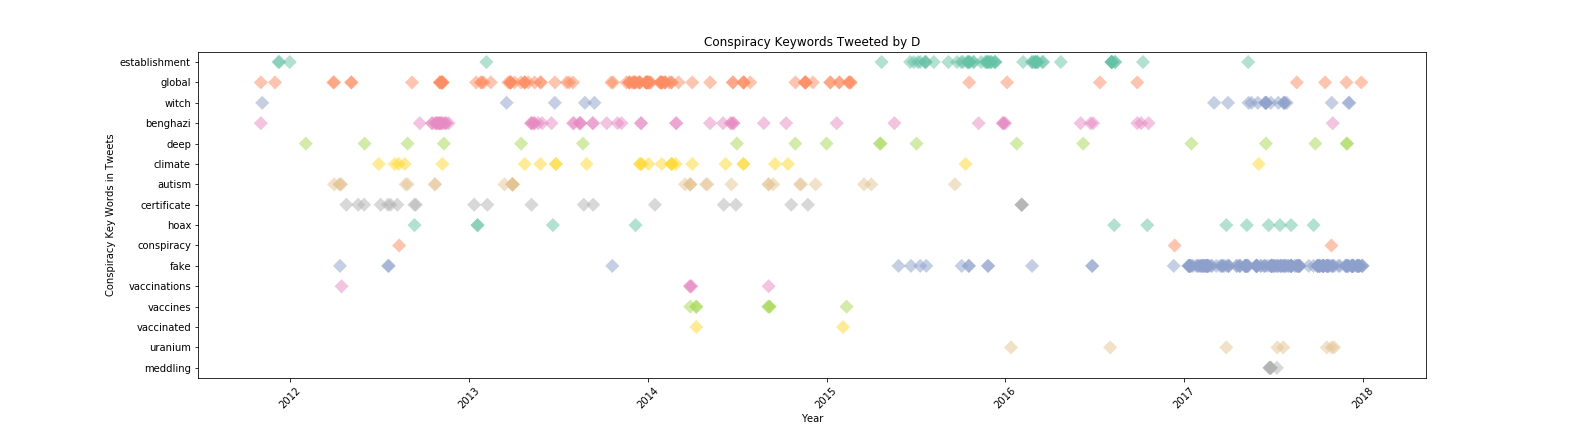
\includegraphics[width=1\textwidth]{figures/Lexical_Dispersion.png}
        \caption{\label{fig:Lexical}Dispersión Léxica de Tweets de Donald Trump} Fuente: Tutorial: Plotting Lexical Dispersion (Conspiracy Lies from the Left-of-Center) \cite{Lexical_Dispersion}
    \end{figure}
    
     En general dentro de los gráficos de dispersión léxica, el eje X puede ser un conjunto de documentos, tal como en el ejemplo recién estudiado, o un único documento en dónde el eje X pasaría a representar la temporalidad de dicho documento.
     
    \item \textbf{Distribución de frecuencias de n-gramas}:
        de la misma forma en que se pudo ver como varía la cantidad de menciones sobre un n-grama a lo largo del tiempo, también es posible ver cómo se distribuye la frecuencia de menciones de n-gramas en un documento particular. Para ello, simplemente se puede construir un gráfico de barras, en donde la altura de cada barra, representa la frecuencia de los n-gramas a analizar. A modo de ejemplo (Ver figura \ref{fig:DistribucionNgramas}), se puede ver la distribución de n-gramas de un documento en particular. Analizando esto, se puede ver que el texto habla sobre videojuegos debido a los conceptos que aparecen como más relevantes.
     \begin{figure}[h!]
        \centering
        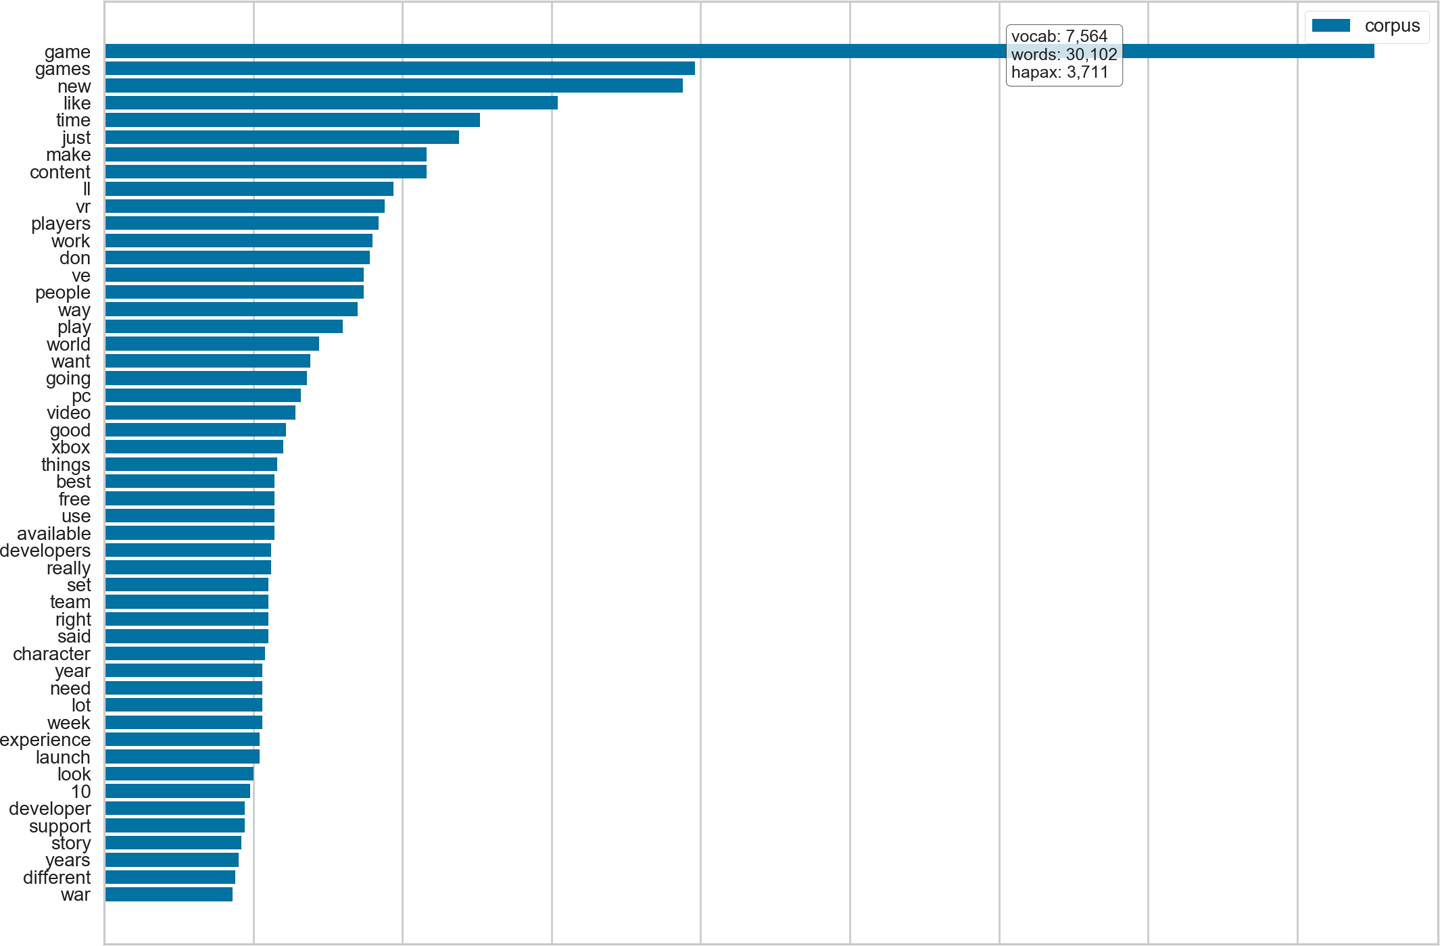
\includegraphics[width=0.8\textwidth]{figures/Distribucion.png}
        \caption{\label{fig:DistribucionNgramas} Distribución de frecuencia de n-gramas} Fuente: Applied text analysis with python \cite{bengfort2018applied}
    \end{figure}
    \item \textbf{Nube de Palabras}: otra forma de visualizar la frecuencia de las palabras es por medio del uso de nubes de palabras (ver figura \ref{fig:WordClouds}). Dentro de una nube de palabras se pueden ver los principales 1-gramas en distintos colores y tamaño. En general el tamaño es proporcional a la frecuencia de la palabra dentro del texto.
    \begin{figure}[H]
        \centering
        
\includegraphics[width=0.8\textwidth]{figures/Word-Cloud.png}
        \caption{\label{fig:WordClouds} Nube de Palabras} Fuente: Generating WordClouds in Python \cite{Word_Clouds}
    \end{figure}
\end{enumerate}
\subparagraph{Visualización  de entidades}
\subparagraph*{}
    Una de las tareas más comunes en proyectos de minería de textos es la identificación de las entidades nombradas dentro de un documento. A continuación se presentan algunas de las técnicas más comunes en este ámbito:
\begin{enumerate}
    \item Matriz de Co-Ocurrencias: indica de forma cualitativa cuantas veces coexisten dos entidades dentro de un mismo documento. A modo de ejemplo se puede ver la cantidad de co-ocurrencias entre los personajes del libro Mago de Oz (ver figrua \ref{fig:MatrizCoOcurrencias}). Además, como se puede apreciar se muestran dos matrices una ordenando los personajes por cantidad de menciones dentro de la obra y otra ordenando los personajes de forma cualitativa.  
    \begin{figure}[H]
        \centering
        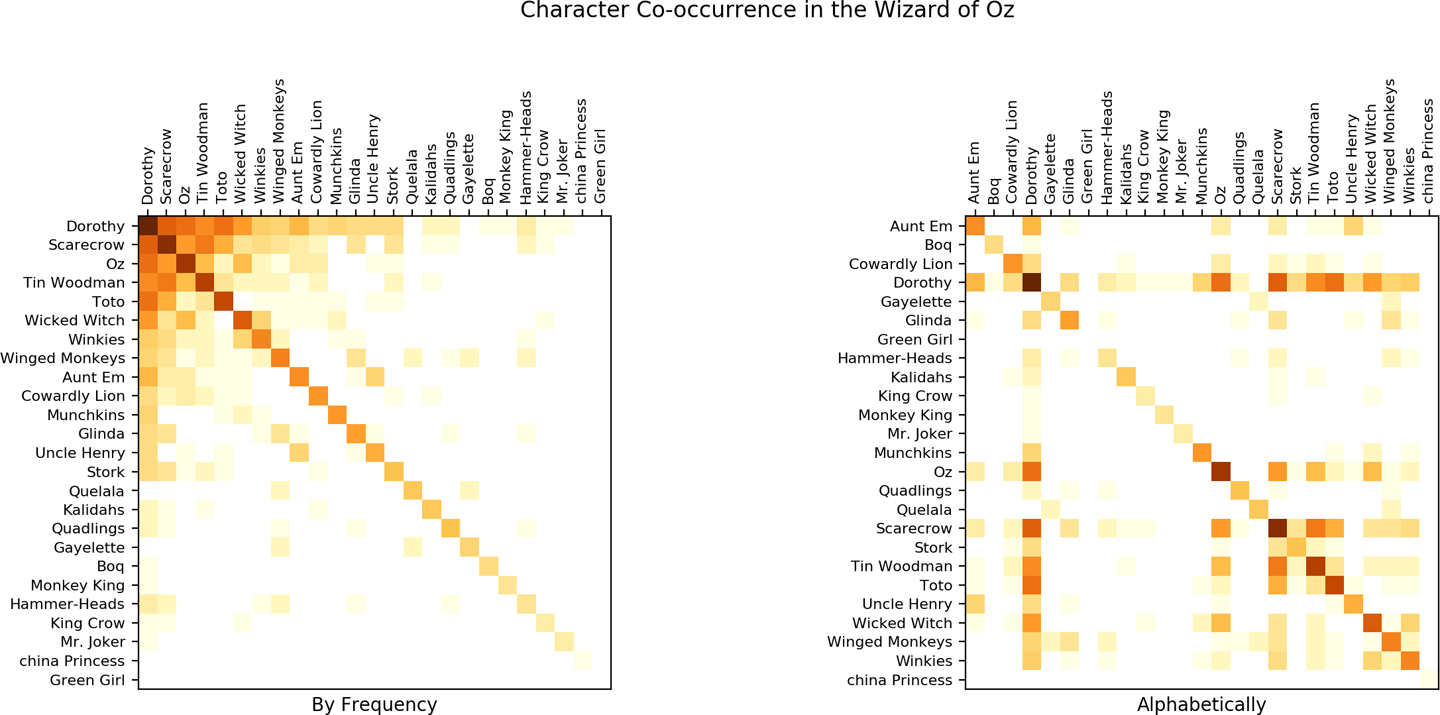
\includegraphics[width=0.8\textwidth]{figures/MatrizCoOcurrencias.png}
        \caption{\label{fig:MatrizCoOcurrencias} Matriz de Co-Ocurrencias del libro Mago de Oz} Fuente: Applied text analysis with python \cite{bengfort2018applied}
    \end{figure}
    \item Gráfico de dispersión: mientras la matriz de co-ocurrencias da una vista general de las relaciones que pueden existir entre personajes, ésta no toma en cuenta cómo una entidad interactúa a lo largo de la narrativa. Los gráficos de dispersión muestran como cierta entidad es nombrada a lo largo del tiempo y, en general, permiten ver en que momentos de un texto cierta entidad es más o menos relevante (ver figrua \ref{fig:DispersionPLot}).
    \begin{figure}[H]
        \centering
        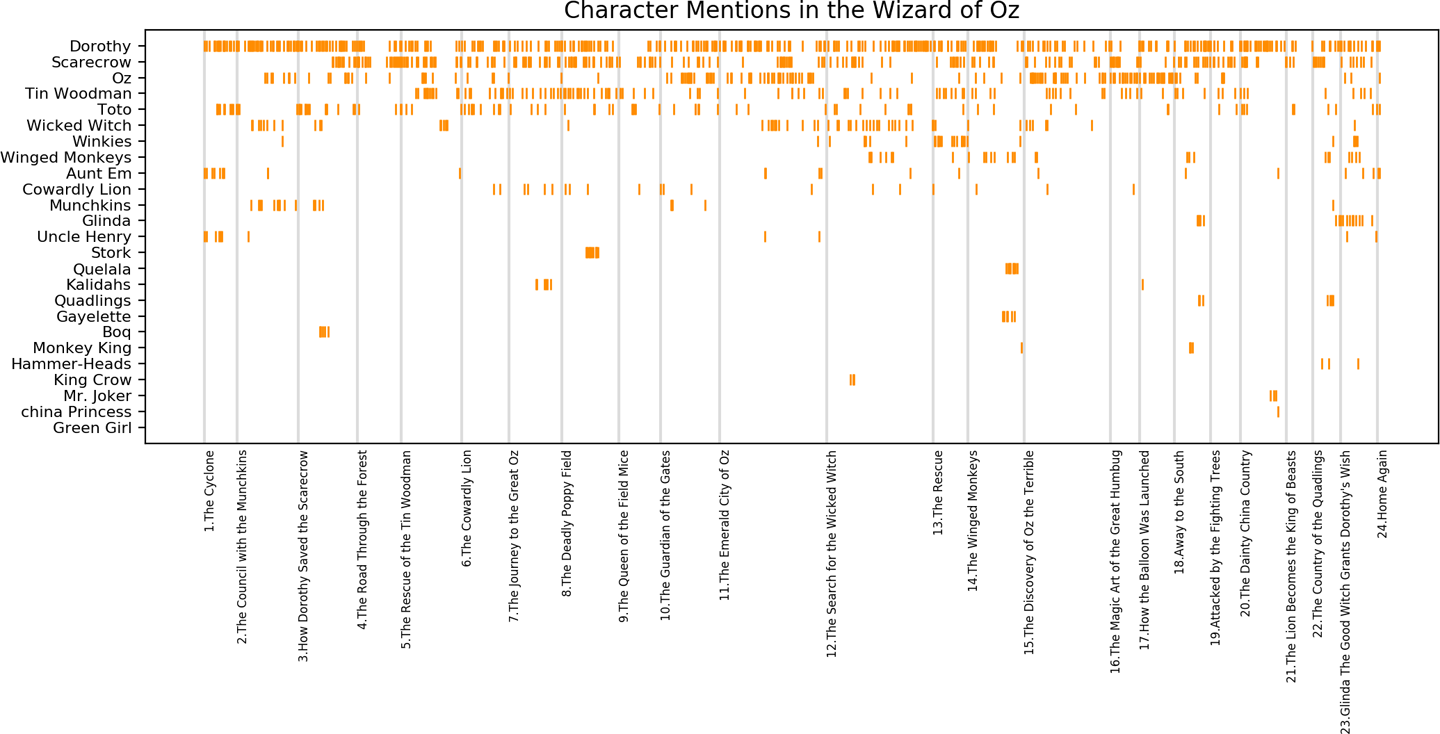
\includegraphics[width=0.8\textwidth]{figures/DispersionPlot.png}
        \caption{\label{fig:DispersionPLot} Gráfico de Dispersión del libro Mago de Oz} Fuente: Applied text analysis with python \cite{bengfort2018applied}
    \end{figure}
\end{enumerate}

\paragraph{Visualización de temas de un corpus de documentos}
    Como se discutió en secciones anteriores, uno de las tareas más comunes a la hora de analizar textos es descubrir los temas latentes que habla un corpus en particular. Sin embargo, comunicar este resultado no es para nada trivial por lo que en la literatura se han desarrollado algunas herramientas que permiten visualizar de mejor forma los resultados de dichos algoritmos.
\subparagraph{LDAvis}
\subparagraph{}*
    LDAvis \cite{sievert2014ldavis} es un sistema web utilizado para visualizar los resultados del algoritmo LDA. LDAVis  busca responder tres preguntas: 
    \begin{enumerate}
        \item ¿Cuál es el significado de cada tema encontrado?
        \item ¿Qué tan frecuente es cada tema dentro del corpus de documentos?
        \item ¿Qué relación y que cosas en común existen entre cada tema encontrado?
    \end{enumerate}
    Para resolver esas tres interrogantes LDAVis (ver figura \ref{fig:LDAVis} ) se compone de dos paneles. El panel izquierdo da una vista global de como se distribuyen los temas, lo que nos ayuda a responder las preguntas 2 y 3. En esta vista se plotean los temas como círculos en dónde el radio de cada círculo está relacionado al porcentaje de \textit{tokens} del \textit{corpus} que pertenecen al tema encontrado (pregunta 2). Además la posición de cada tema es calculada según la distancia entre temas y luego cada tema es proyectado utilizando PCA a dos dimensiones (pregunta 3). 
    
    Por otro lado el panel derecho de la visualización entrega un diagrama de barras horizontal que representan a los 30 términos más relevantes para el tema seleccionado en el panel izquierdo (pregunta 1).
    \begin{figure}[H]
        \centering
        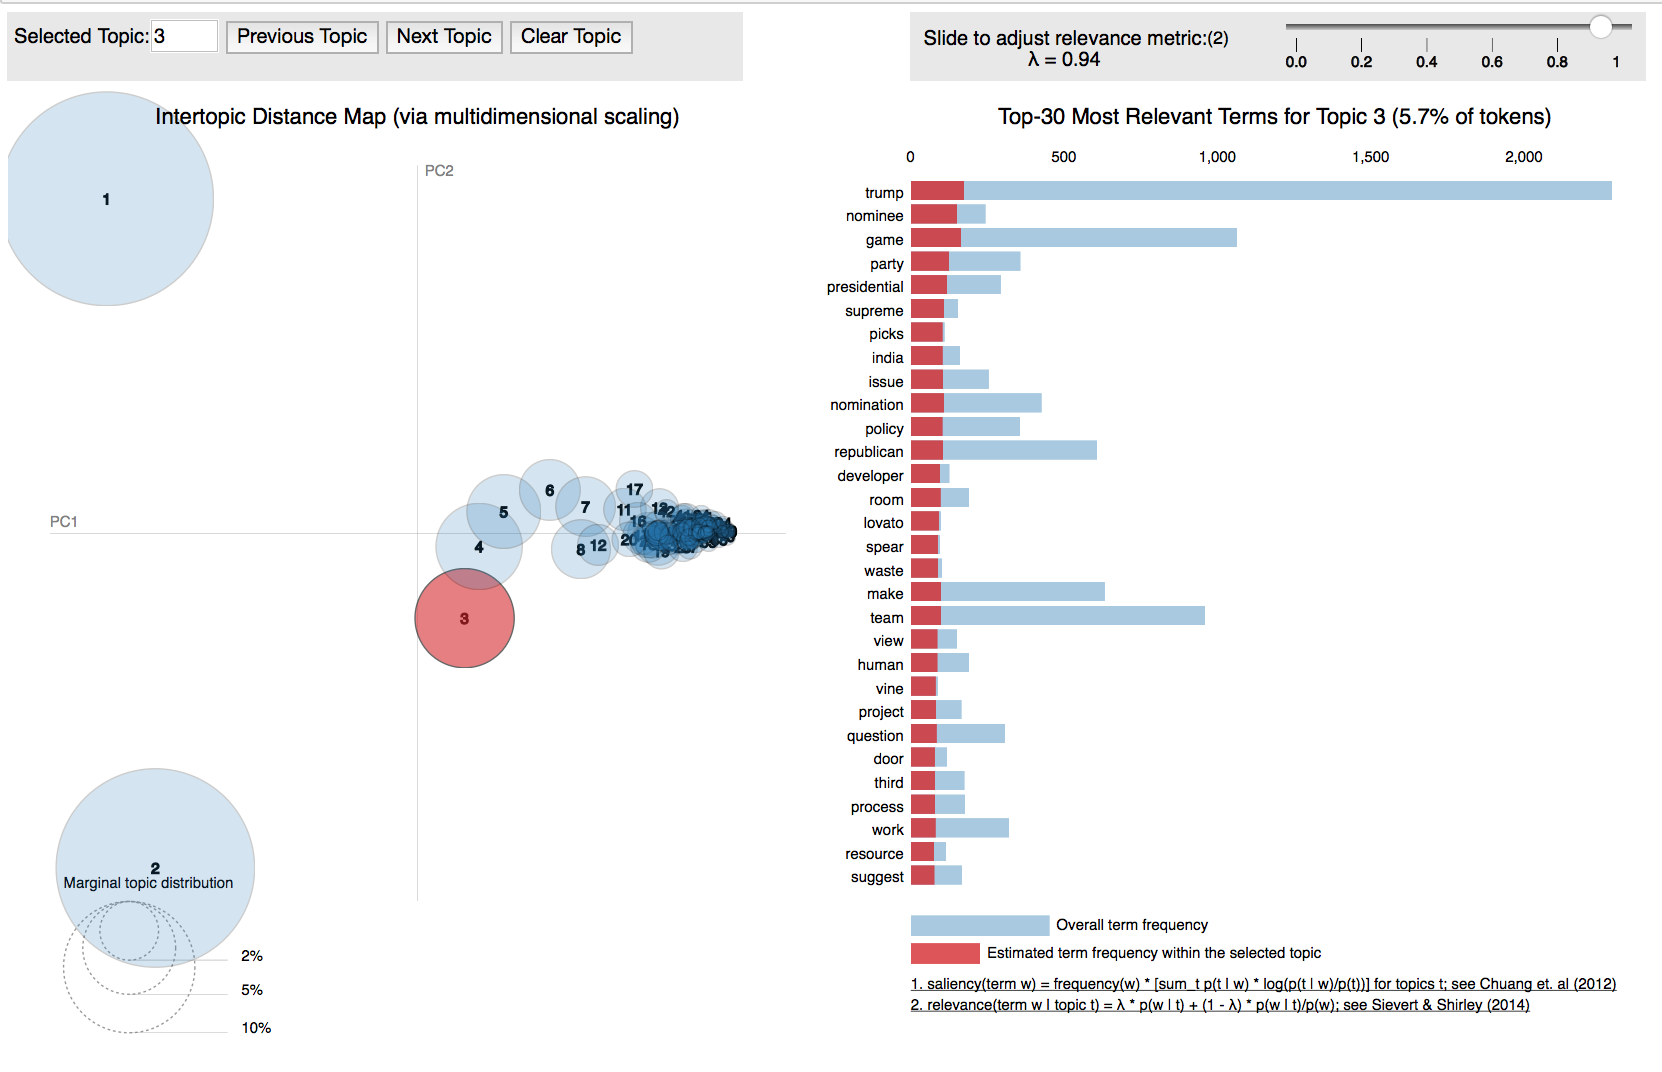
\includegraphics[width=0.8\textwidth]{figures/LDAVis.png}
        \caption{\label{fig:LDAVis} LDAVis} Fuente: LDAvis: A method for visualizing and interpreting topics \cite{sievert2014ldavis}
    \end{figure}
\subparagraph{Visualización para LDA}
\subparagraph*{}
    Otra forma de visualizar los temas extraídos de cierto \textit{corpus} de documentos fue planteado en \cite{kucher2018analysis}. Esta visualización es utilizada para demostrar los resultados de extracción de temas utilizando el algoritmo LDA, y se basa en la visualización LDAVis descrita anteriormente. 
    
   Se compone de tres paneles, denotados por a), b) y c) en la figura 14 que sirve de ejemplo. A continuación se describen los tres paneles por separado:
    
    \begin{itemize}
        \item Panel a) : es un \textit{scatterplot} en dónde cada punto es uno de los documentos analizados. Cada uno estos posee N-\textit{Features} que corresponden a la probabilidad de cada documento de pertenecer a uno de los N tópicos encontrados por LDA. El espacio de N temas es reducido a dos utilizando t-SNE y sobre ese nuevo espacio reducido son proyectados los documentos permitiendo visualizar \textit{clusters} de documentos, en este caso los 7 temas más relevantes dentro del \textit{corpus} analizado. Otra cosa que se puede ver en este panel son los colores de cada punto. En este caso el color opaco implica que existe una alta probabilidad del documento de pertenecer al tema asignado mientras que un color transparente nos dice lo contrario.
        
        \item Panel b): es un \textit{barchart} que nos muestra el porcentaje de términos pertenecientes a cada uno de los tópiocs encontrados por nuestro algoritmo.
        
        \item Panel c): muestra los términos más relevantes para el tema seleccionado en el panel b. Además, entre paréntesis índica la cantidad de veces que aparece el término en dicho tema. Finalmente el color de la barra muestra a qué tema está más relacionado el término en cuestión.
    \end{itemize}
    
    \begin{figure}[H]
        \centering
        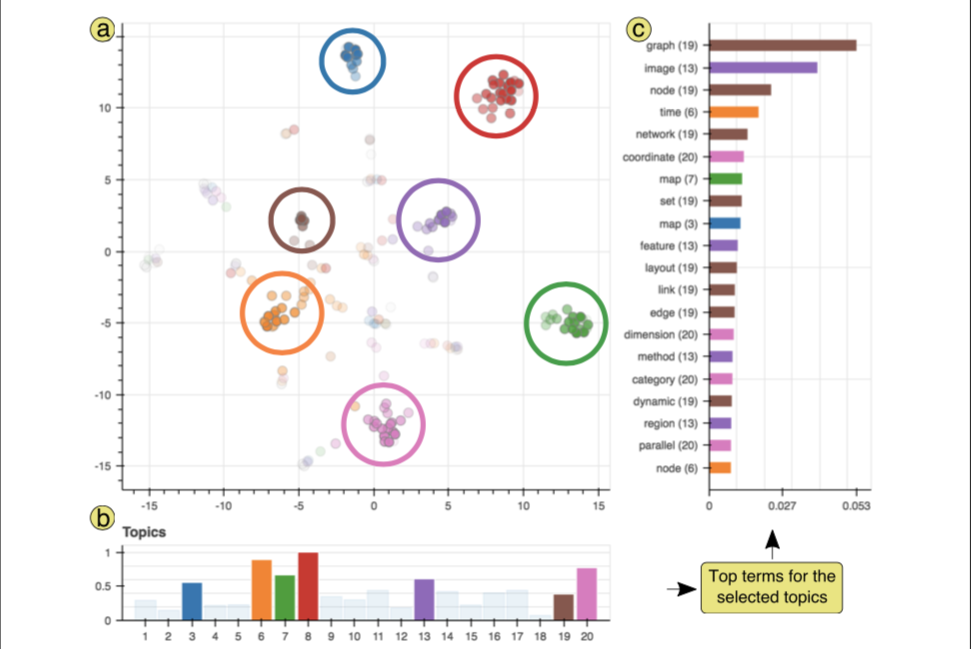
\includegraphics[width=0.8\textwidth]{figures/AnalisisVinci.png}
        \caption{\label{fig:Vinci} Visualización para LDA} Fuente: Analysis of VINCI 2009–2017 Proceedings \cite{kucher2018analysis}
    \end{figure}
    
\paragraph{Visualización de clusters de documentos}
\subparagraph{Visualización para Clustering jerarquico aglomerativo}
\subparagraph*{}
    El proceso de clustering jerárquico aglomerativo puede ser resumido en un \textit{Dendrograma} \cite{everitt1998cambridge}. Este árbol ilustra la serie de pasos que toma el método para formar desde n clusters un único gran cluster que contiene todos los datos analizados (Ver figura \ref{fig:Dendrogram}). 

    \begin{figure}[H]
        \centering
        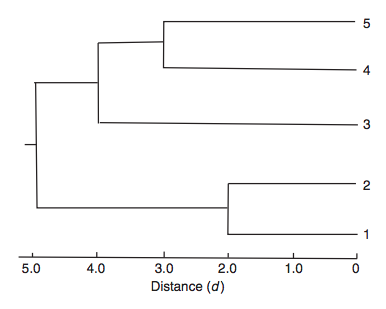
\includegraphics[width=0.8\textwidth]{figures/Dendrogram.png}
        \caption{\label{fig:Dendrogram} Dendrograma} Fuente: 
        The cambridge dictionary of statistics cambridge university press \cite{everitt1998cambridge}
    \end{figure}
    


